% 矩阵方程：Sylvester方程AX+XB=C（线性算子与向量化、谱条件、Bartels--Stewart求解、可对角化情形）；
% Lyapunov方程X-A^TXA=Q与AX+XA^T=Q（离散累计与唯一性、保持结构的Schur求解、级数解与正定性）

\section{Sylvester方程}
\label{sec:ls-matrix-equations}

前面各节的未知量都是向量。若未知量是一张矩阵$\bm X$，并且同时受到已知矩阵的左乘和右乘，怎样判断方程可解，又怎样在保持矩阵形状的前提下算出解？
本节从$\bm A\bm X=\bm C$、$\bm A\bm X\bm B=\bm C$进入$\bm A\bm X+\bm X\bm B=\bm C$，先用向量化确认它仍是线性问题，再用第~\ref{sec:ls-general-square-spectrum}节的谱与实Schur形给出可解条件和求解路线。
可解性看的是线性算子是否可逆，计算则利用它的左右结构；形成巨大的Kronecker系数矩阵不是默认算法。

\subsection{矩阵未知量与线性算子}
\label{sec:ls-matrix-equation-types}

已知矩阵从左边、右边或两边作用在未知矩阵上，这样的方程称为\term{矩阵方程}（matrix equation）。单侧方程$\bm A\bm X=\bm C$是共用系数的多右端线性方程；双侧方程$\bm A\bm X\bm B=\bm C$在两侧系数可逆时，可以先左乘$\bm A^{-1}$、再右乘$\bm B^{-1}$，两次“除法”互不干扰。本节研究左右两种作用相加的\term{Sylvester方程}（Sylvester equation）
\[
 \bm A\bm X+\bm X\bm B=\bm C,
\]
其中$\bm A\in\mathbb R^{m\times m}$、$\bm B\in\mathbb R^{d\times d}$、$\bm C\in\mathbb R^{m\times d}$，未知量$\bm X\in\mathbb R^{m\times d}$。$\bm A$作用在$\bm X$的列上，阶数等于$\bm X$的行数；$\bm B$作用在$\bm X$的行上，阶数等于$\bm X$的列数。两项相加以后就不能分别“除以”两个系数：左乘$\bm A^{-1}$只得到$\bm X+\bm A^{-1}\bm X\bm B=\bm A^{-1}\bm C$，未知量仍同时出现在两项中。

左边$\mathcal L(\bm X)=\bm A\bm X+\bm X\bm B$由矩阵乘法的分配律对$\bm X$是线性的，所以Sylvester方程就是$md$维空间$\mathbb R^{m\times d}$上的线性方程$\mathcal L(\bm X)=\bm C$。把矩阵按列拉直，由第~\ref{sec:ls-kronecker-products}节的恒等式$\operatorname{vec}(\bm A\bm X\bm B)=(\bm B^\top\otimes\bm A)\operatorname{vec}\bm X$，把$\bm A\bm X$看成$\bm A\bm X\bm I_d$、把$\bm X\bm B$看成$\bm I_m\bm X\bm B$，相加得
\begin{equation}
 (\bm I_d\otimes\bm A+\bm B^\top\otimes\bm I_m)\operatorname{vec}\bm X
 =\operatorname{vec}\bm C .
 \label{eq:ls-sylvester-vectorized}
\end{equation}
记系数矩阵为$\bm K\in\mathbb R^{md\times md}$。这一表达说明前面关于线性方程的判据都适用，也适合用LU分解（第~\ref{sec:ls-lu}节）核验小例子。但$\bm K$有$(md)^2$个元素，$m=d=100$时已达$10^8$个，稠密消元约需$\tfrac23(md)^3$次运算；大规模求解应保留矩阵形状。

\subsection{存在唯一性的谱条件}
\label{sec:ls-matrix-equation-existence}

单侧方程可以直接沿用列空间判据：$\bm A\bm X=\bm C$相容，当且仅当$\bm C$的每一列都在$\operatorname{range}(\bm A)$中，即$\operatorname{rank}[\bm A\ \bm C]=\operatorname{rank}(\bm A)$。双侧方程的相容性由向量化方程$(\bm B^\top\otimes\bm A)\operatorname{vec}\bm X=\operatorname{vec}\bm C$的增广秩判据判断。两侧系数都可逆时，唯一解为$\bm X=\bm A^{-1}\bm C\bm B^{-1}$；任一侧秩亏时，方程可能无解，有解时也可以沿该侧的零空间变动，因而不唯一。

Sylvester方程不能这样逐侧处理，对角情形能看出原因。设$\bm A=\operatorname{diag}(\lambda_1,\ldots,\lambda_m)$、$\bm B=\operatorname{diag}(\mu_1,\ldots,\mu_d)$，则$\bm A\bm X$把第$i$行乘以$\lambda_i$，$\bm X\bm B$把第$j$列乘以$\mu_j$，方程按元素分解为$(\lambda_i+\mu_j)x_{i,j}=c_{i,j}$，分母非零时
\begin{equation}
 x_{i,j}=\frac{c_{i,j}}{\lambda_i+\mu_j}.
 \label{eq:ls-sylvester-diagonal-closed-form}
\end{equation}
若某个$\lambda_i+\mu_j=0$，该位置退化为$0\cdot x_{i,j}=c_{i,j}$：$c_{i,j}\neq0$时无解，$c_{i,j}=0$时$x_{i,j}$可以任取。所以决定可解性的是$\bm A$的特征值与$-\bm B$的特征值是否重合（图~\ref{fig:ls-sylvester-separation}）。一般情形的结论相同，只是实矩阵的特征值可能是复数，条件要在复数域中检查。下面记$\operatorname{spec}(\bm A)$为$\bm A$在复数域中的全体特征值。

\begin{figure}[htbp]
  \centering
  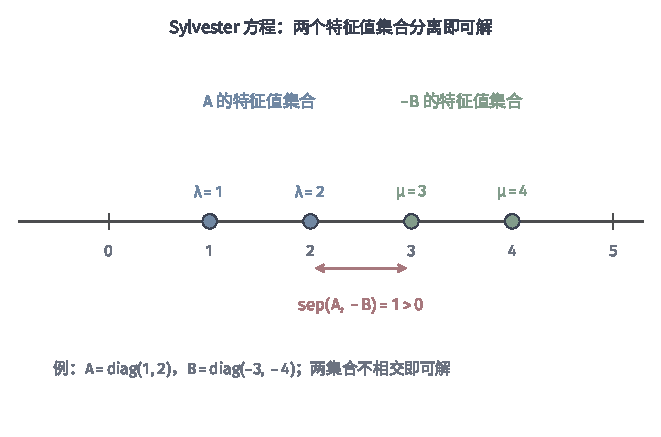
\includegraphics[width=112mm]{figures/00-shared/mathematical-preliminaries-upper/02-linear-spaces/matplotlib/ls-sylvester-separation/ls-sylvester-separation.pdf}
  \caption{谱分离条件的实轴示意。$\bm A=\operatorname{diag}(1,2)$的特征值$\{1,2\}$与$-\bm B$（$\bm B=\operatorname{diag}(-3,-4)$）的特征值$\{3,4\}$不相交，最近一对相距$1$，所以四个分母$\lambda_i+\mu_j$都不为零，对任意$\bm C$方程都有唯一解。}
  \label{fig:ls-sylvester-separation}
\end{figure}

\begin{theorem}[Sylvester方程的唯一可解性]
\label{thm:ls-sylvester-unique-solvability}
设$\bm A\in\mathbb R^{m\times m}$、$\bm B\in\mathbb R^{d\times d}$。方程$\bm A\bm X+\bm X\bm B=\bm C$对每个$\bm C\in\mathbb R^{m\times d}$都有唯一解，当且仅当
\begin{equation}
 \operatorname{spec}(\bm A)\cap\operatorname{spec}(-\bm B)=\varnothing ,
 \label{eq:ls-sylvester-spectral-separation}
\end{equation}
即对$\bm A$的任一特征值$\lambda$与$\bm B$的任一特征值$\mu$，都有$\lambda+\mu\neq0$。
\end{theorem}

\begin{proof}
$\mathcal L$把$\mathbb R^{m\times d}$映到自身，由秩零度定理，它对每个右端唯一可解当且仅当齐次方程只有零解，也就是$\det\bm K\neq0$。这个行列式在实数域和复数域中是同一个数，所以可以在复数域中讨论齐次方程。

必要性。若$\bm A\bm u=\lambda\bm u$，且$-\lambda$是$\bm B$的特征值，则$-\lambda$也是$\bm B^\top$的特征值，取$\bm B^\top\bm w=-\lambda\bm w$，其中$\bm u,\bm w\neq\bm0$。$\bm X=\bm u\bm w^\top\neq\bm0$满足$\bm A\bm X+\bm X\bm B=\lambda\bm u\bm w^\top-\lambda\bm u\bm w^\top=\bm0$。

充分性。设$\bm A\bm X=\bm X(-\bm B)$，归纳得$\bm A^k\bm X=\bm X(-\bm B)^k$，从而对任意多项式$p$有$p(\bm A)\bm X=\bm X\,p(-\bm B)$。取$p(z)=\prod_k(z-\lambda_k)$为$\bm A$的特征多项式，由Cayley--Hamilton定理~\ref{thm:ls-cayley-hamilton}，$p(\bm A)=\bm0$；而$p(-\bm B)=\prod_k(-\bm B-\lambda_k\bm I)$中每个$\lambda_k$都不是$-\bm B$的特征值，各因子可逆。于是$\bm X\,p(-\bm B)=\bm0$推出$\bm X=\bm0$。
\end{proof}

这一条件与$\bm A$、$\bm B$各自是否可逆无关。$\bm A=\bm0$、$\bm B=\bm I_d$时$\bm A$不可逆，方程却化为$\bm X=\bm C$，唯一可解；$1\times1$情形$\bm A=2$、$\bm B=-2$都可逆，方程却是$0\cdot x=c$。谱不相交只回答解是否唯一，不回答解对数据误差是否敏感：对角情形下最小的$|\lambda_i+\mu_j|$越接近零，$\bm C$的误差放大越多；矩阵远离正规时，即使所有谱和都远离零，解仍可能很敏感，第~\ref{sec:ls-sylvester-diagonalizable}节会看到其中的原因。

\subsection{基于Schur分解的求解}
\label{sec:ls-sylvester-schur}

稠密的一般Sylvester方程通常用Bartels--Stewart算法求解。它的思路与解三角方程组相同：先用正交相似把两个系数化为准上三角形，方程的未知元之间就有了先后依赖，可以按列逐个回代；正交变换既不改变特征值，也不改变残差大小。下面设谱条件~\eqref{eq:ls-sylvester-spectral-separation}成立。

\paragraph{实Schur分解}
第一步，分别对两个系数作实Schur分解（定理~\ref{thm:ls-real-schur}）
\[
 \bm A=\bm U\bm T\bm U^\top,\qquad \bm B=\bm V\bm S\bm V^\top,
\]
其中$\bm U,\bm V$正交，$\bm T,\bm S$是准上三角矩阵，对角块为$1\times1$（实特征值）或$2\times2$（一对共轭复特征值）。这一步只依赖$\bm A$、$\bm B$，与右端无关。

\paragraph{变换右端与未知量}
方程两边左乘$\bm U^\top$、右乘$\bm V$，利用$\bm U^\top\bm A=\bm T\bm U^\top$与$\bm B\bm V=\bm V\bm S$，并记$\bm Y=\bm U^\top\bm X\bm V$、$\bm D=\bm U^\top\bm C\bm V$，方程化为
\begin{equation}
 \bm T\bm Y+\bm Y\bm S=\bm D .
 \label{eq:ls-sylvester-transformed}
\end{equation}
$\bm T$与$\bm A$、$\bm S$与$\bm B$的特征值相同，所以新方程同样满足谱条件。

\paragraph{逐列求解\texorpdfstring{$\bm Y$}{Y}}
先看$\bm T$、$\bm S$都是上三角的情形。$\bm Y\bm S$的第$j$列是$\sum_{\ell\leq j}s_{\ell,j}\bm y_\ell$，比较式~\eqref{eq:ls-sylvester-transformed}两边的第$j$列，把含$\bm y_j$的项留在左边，得
\[
 (\bm T+s_{j,j}\bm I_m)\bm y_j=\bm d_j-\sum_{\ell<j}s_{\ell,j}\bm y_\ell .
\]
右端只用到更靠左的列，所以按$j=1,\ldots,d$从左到右计算；每列的系数仍是上三角矩阵，用第~\ref{sec:ls-lu}节的回代从最后一行向上求解，除数$t_{i,i}+s_{j,j}$是$\bm A$与$\bm B$的一对特征值之和，由谱条件不为零。图~\ref{fig:ls-bartels-stewart-column-order}画出了第$j$列的依赖：$\bm S$第$j$列中对角线以上的元素把已求出的列带进右端，对角元$s_{j,j}$并入当前列的三角系数。

\begin{figure}[htbp]
  \centering
  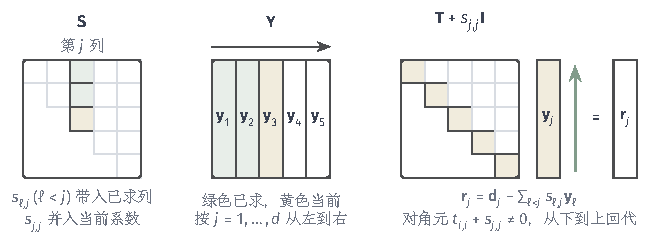
\includegraphics[width=109.6mm]{figures/01-basic-mathematics/03-vectors-matrices-and-multivariate-functions/tikz/c5-bartels-stewart-column-order/figure.pdf}
  \caption{Bartels--Stewart算法逐列求解$\bm T\bm Y+\bm Y\bm S=\bm D$的次序（上三角情形，图中取当前列$j=3$）。左：$\bm S$的第$j$列，绿色元素$s_{\ell,j}$（$\ell<j$）对应已求出的列，黄色为$s_{j,j}$。中：$\bm Y$的列从左到右求出。右：当前列解一个对角元为$t_{i,i}+s_{j,j}$的上三角方程组，从最后一行向上回代。}
  \label{fig:ls-bartels-stewart-column-order}
\end{figure}

含$2\times2$块时，把$\bm Y$、$\bm D$按$\bm T$、$\bm S$的对角块分块，比较第$(i,j)$块得
\[
 \begin{aligned}
 \bm T_{i,i}\bm Y_{i,j}+\bm Y_{i,j}\bm S_{j,j}
 &=\bm D_{i,j}-\sum_{k>i}\bm T_{i,k}\bm Y_{k,j}\\
 &\quad-\sum_{\ell<j}\bm Y_{i,\ell}\bm S_{\ell,j}.
 \end{aligned}
\]
右端只含同一块列中更靠下的块和更靠左的块列，因此按块列从左到右、每块列从下到上计算。左边是至多含四个未知量的小Sylvester方程，用式~\eqref{eq:ls-sylvester-vectorized}化为至多$4$阶的方程直接消元即可。

\paragraph{恢复原未知量}
最后令$\bm X=\bm U\bm Y\bm V^\top$，并在原方程中计算残差$\bm A\bm X+\bm X\bm B-\bm C$。精确算术下它为零；浮点计算中它的Frobenius范数与新坐标中的残差相同（见下面的定理），因此可以直接用来检验整个流程。

\begin{example}[Bartels--Stewart求解一个二阶方程]
\label{ex:ls-bartels-stewart-2x2}
取
\[
 \bm A=\begin{bmatrix}-2&3\\-4&5\end{bmatrix},\quad
 \bm B=\begin{bmatrix}1&1\\0&3\end{bmatrix},\quad
 \bm C=\begin{bmatrix}1&12\\-2&21\end{bmatrix}.
\]
$\bm A$的特征值为$2,1$，$-\bm B$的特征值为$-1,-3$，谱条件成立。实Schur分解：由$\bm A(3,4)^\top=2(3,4)^\top$取$\bm U=\tfrac15\bigl[\begin{smallmatrix}3&-4\\4&3\end{smallmatrix}\bigr]$，得$\bm T=\bm U^\top\bm A\bm U=\bigl[\begin{smallmatrix}2&7\\0&1\end{smallmatrix}\bigr]$；$\bm B$已是上三角，取$\bm V=\bm I$、$\bm S=\bm B$。变换右端得$\bm D=\bm U^\top\bm C=\bigl[\begin{smallmatrix}-1&24\\-2&3\end{smallmatrix}\bigr]$。

逐列求解：第$1$列解$(\bm T+s_{1,1}\bm I)\bm y_1=\bm d_1$，即$\bigl[\begin{smallmatrix}3&7\\0&2\end{smallmatrix}\bigr]\bm y_1=(-1,-2)^\top$，从下往上得$y_{2,1}=-1$、$y_{1,1}=2$；第$2$列的右端为$\bm d_2-s_{1,2}\bm y_1=(24,3)^\top-(2,-1)^\top=(22,4)^\top$，解$\bigl[\begin{smallmatrix}5&7\\0&4\end{smallmatrix}\bigr]\bm y_2=(22,4)^\top$得$y_{2,2}=1$、$y_{1,2}=3$。变回原坐标，
\[
 \bm X=\bm U\bm Y=\frac15\begin{bmatrix}3&-4\\4&3\end{bmatrix}\begin{bmatrix}2&3\\-1&1\end{bmatrix}=\begin{bmatrix}2&1\\1&3\end{bmatrix}.
\]
核验：$\bm A\bm X=\bigl[\begin{smallmatrix}-1&7\\-3&11\end{smallmatrix}\bigr]$，$\bm X\bm B=\bigl[\begin{smallmatrix}2&5\\1&10\end{smallmatrix}\bigr]$，和为$\bm C$，残差为零。
\end{example}

\paragraph{正确性}
上面的推导说明每一步都能进行，而且按次序算出的块满足各自的块等式。把这些事实合在一起，就得到算法的正确性和残差检验的依据。

\begin{theorem}[Bartels--Stewart算法的正确性]
\label{thm:ls-bartels-stewart}
设$\bm A=\bm U\bm T\bm U^\top$、$\bm B=\bm V\bm S\bm V^\top$是实Schur分解，谱条件~\eqref{eq:ls-sylvester-spectral-separation}成立，$\bm D=\bm U^\top\bm C\bm V$。则
\begin{enumerate}
 \item 按块列从左到右、每块列从下到上的次序，每一步的局部方程$\bm T_{i,i}\bm Y_{i,j}+\bm Y_{i,j}\bm S_{j,j}=\bm E_{i,j}$都唯一可解，其中右端$\bm E_{i,j}$由已求出的块给出；
 \item 由此算出的$\bm Y$是方程~\eqref{eq:ls-sylvester-transformed}的唯一解，$\bm X=\bm U\bm Y\bm V^\top$是$\bm A\bm X+\bm X\bm B=\bm C$的唯一解；
 \item 对任意$\bm Z\in\mathbb R^{m\times d}$，记$\bm W=\bm U^\top\bm Z\bm V$，有$\lVert\bm A\bm Z+\bm Z\bm B-\bm C\rVert_{\mathrm F}=\lVert\bm T\bm W+\bm W\bm S-\bm D\rVert_{\mathrm F}$。
\end{enumerate}
\end{theorem}

\begin{proof}
先证第三条。由$\bm A=\bm U\bm T\bm U^\top$、$\bm B=\bm V\bm S\bm V^\top$与$\bm Z=\bm U\bm W\bm V^\top$，
\[
 \bm A\bm Z+\bm Z\bm B-\bm C=\bm U(\bm T\bm W+\bm W\bm S-\bm D)\bm V^\top,
\]
而左右乘正交矩阵不改变Frobenius范数。

再证第一条。准上三角矩阵的特征值是各对角块特征值的并，$\bm T$与$\bm A$相似，所以$\bm T_{i,i}$的特征值都是$\bm A$的特征值；同理$\bm S_{j,j}$的特征值都是$\bm B$的特征值。于是每个局部方程满足谱条件，由定理~\ref{thm:ls-sylvester-unique-solvability}唯一可解。

最后证第二条。第$(i,j)$块等式的右端只含按次序已算出的块，所以算出的每一块都满足相应的块等式；全部块等式合起来就是式~\eqref{eq:ls-sylvester-transformed}。$\bm T$、$\bm S$满足谱条件，由定理~\ref{thm:ls-sylvester-unique-solvability}，这个解唯一。在第三条中取$\bm Z=\bm X$、$\bm W=\bm Y$，得原方程残差为零；原方程的唯一性同样由该定理给出。
\end{proof}

\paragraph{计算代价}
实Schur分解靠迭代算出，常用实现计入正交因子约需$25m^3$与$25d^3$次运算\scite{math-golub2013matrix}；变换右端与变回原坐标各约$2(m^2d+md^2)$次，逐列回代约$m^2d+md^2$次；存储只需$O(m^2+d^2+md)$个数。$m=d=100$时总量约$6\times10^7$次，而对式~\eqref{eq:ls-sylvester-vectorized}作稠密LU约需$7\times10^{11}$次，并要存储$10^8$个数。多组右端共用$\bm A$、$\bm B$时，两个Schur分解只做一次，每增加一个右端只增加$O(m^2d+md^2)$次运算。

\subsection{可对角化系数的特殊情形}
\label{sec:ls-sylvester-diagonalizable}

当$\bm A$、$\bm B$都可对角化时，可以换到各自的特征基，把方程化为对角情形。设$\bm A=\bm P\bm\Lambda\bm P^{-1}$、$\bm B=\bm R\bm M\bm R^{-1}$，其中$\bm\Lambda=\operatorname{diag}(\lambda_i)$、$\bm M=\operatorname{diag}(\mu_j)$。

\paragraph{换到特征基}
记$\bm Y=\bm P^{-1}\bm X\bm R$、$\bm D=\bm P^{-1}\bm C\bm R$。方程左乘$\bm P^{-1}$、右乘$\bm R$，由$\bm P^{-1}\bm A=\bm\Lambda\bm P^{-1}$与$\bm B\bm R=\bm R\bm M$化为$\bm\Lambda\bm Y+\bm Y\bm M=\bm D$。计算$\bm D$时不必求逆：先对$\bm P$作LU分解，对$\bm C$的各列求解$\bm P\bm Z=\bm C$，再令$\bm D=\bm Z\bm R$。

\paragraph{逐元素相除}
对角方程按式~\eqref{eq:ls-sylvester-diagonal-closed-form}逐元素求解，$y_{i,j}=d_{i,j}/(\lambda_i+\mu_j)$，谱条件保证所有分母非零。

\paragraph{恢复原未知量}
次序与换基相反：先算$\bm W=\bm P\bm Y$，再利用$\bm R$的LU分解求解$\bm X\bm R=\bm W$，得$\bm X=\bm P\bm Y\bm R^{-1}$。实矩阵有复特征值时，$\bm P$、$\bm R$为复矩阵，全程用复数运算，最后舍去舍入产生的虚部。

\begin{example}[特征基下的逐元素求解]
\label{ex:ls-sylvester-eigenbasis}
取
\[
 \bm A=\begin{bmatrix}1&1\\0&2\end{bmatrix},\quad
 \bm B=\begin{bmatrix}3&1\\0&4\end{bmatrix},\quad
 \bm C=\begin{bmatrix}7&12\\15&21\end{bmatrix}.
\]
两者的特征向量都是$(1,0)^\top$与$(1,1)^\top$，故$\bm P=\bm R=\bigl[\begin{smallmatrix}1&1\\0&1\end{smallmatrix}\bigr]$，特征值分别为$1,2$与$3,4$，四个分母$\lambda_i+\mu_j$为$4,5,5,6$。换基、逐元素相除、再变回，依次得
\[
 \begin{gathered}
 \bm D=\bm P^{-1}\bm C\bm R=\begin{bmatrix}-8&-17\\15&36\end{bmatrix},\qquad
 \bm Y=\begin{bmatrix}-2&-17/5\\3&6\end{bmatrix},\\
 \bm X=\bm P\bm Y\bm R^{-1}=\begin{bmatrix}1&8/5\\3&3\end{bmatrix}.
 \end{gathered}
\]
代回有$\bm A\bm X=\bigl[\begin{smallmatrix}4&23/5\\6&6\end{smallmatrix}\bigr]$、$\bm X\bm B=\bigl[\begin{smallmatrix}3&37/5\\9&15\end{smallmatrix}\bigr]$，和为$\bm C$，残差为零。若把$\bm B$的$(1,1)$元改为$-2$，则$\mu_1=-2$，$\lambda_2+\mu_1=0$，第$(2,1)$个方程变为$0\cdot y_{2,1}=d_{2,1}$：$d_{2,1}\neq0$时无解，$d_{2,1}=0$时解不唯一。
\end{example}

\paragraph{数值敏感度}
这条路线公式简短，但只在特征基接近正交时可靠。记$\delta_{\min}=\min_{i,j}|\lambda_i+\mu_j|$，则$\lVert\bm Y\rVert_{\mathrm F}\leq\lVert\bm D\rVert_{\mathrm F}/\delta_{\min}$；再对$\bm D=\bm P^{-1}\bm C\bm R$与$\bm X=\bm P\bm Y\bm R^{-1}$使用$\lVert\bm M_1\bm Z\bm M_2\rVert_{\mathrm F}\leq\lVert\bm M_1\rVert_2\lVert\bm Z\rVert_{\mathrm F}\lVert\bm M_2\rVert_2$，只能得到
\[
 \lVert\bm X\rVert_{\mathrm F}
 \leq\frac{\kappa_2(\bm P)\,\kappa_2(\bm R)}{\delta_{\min}}\lVert\bm C\rVert_{\mathrm F},
\]
所以谱和远离零在斜基下并不独自保证良好条件。换基本身也会放大误差：$\bm P^{-1}\bm C$的元素可以比$\bm C$大$\kappa_2(\bm P)$量级，变回时再相互抵消。例如$0<\epsilon\ll1$时，$\bm A=\bigl[\begin{smallmatrix}1&1\\0&1+\epsilon\end{smallmatrix}\bigr]$的特征向量$(1,0)^\top$与$(1,\epsilon)^\top$几乎平行，$\kappa_2(\bm P)\geq1/\epsilon$，中间量的大小约为$1/\epsilon$，舍入误差随之被放大。$\bm A$、$\bm B$实对称时，谱定理~\ref{thm:ls-real-symmetric-spectral}给出正交特征基，$\kappa_2=1$，元素公式既简单又可靠；一般情形即使可以对角化，也宜使用第~\ref{sec:ls-sylvester-schur}节的正交Schur变换。

\section{Lyapunov方程}
\label{sec:ls-lyapunov}

第~\ref{sec:ls-convergence}节研究了反复作用$\bm x_{k+1}=\bm A\bm x_k$的长期行为。若每一步以$\bm x_k^\top\bm Q\bm x_k$计量状态的大小，能否用一个矩阵$\bm X$直接写出全部步骤的累计量$\bm x_0^\top\bm X\bm x_0$？本节由这一离散累计引出Lyapunov方程，再讨论相应的连续型方程，然后给出保持对称结构的求解方法与正定解的条件。离散型的论证只用矩阵幂和级数；连续型正定解的积分证明，留到矩阵指数与无穷积分的工具齐备之后。

\subsection{离散型与连续型方程}
\label{sec:ls-lyapunov-solvability}

设$\bm A\in\mathbb R^{d\times d}$，$\bm Q=\bm Q^\top\succeq0$，$\bm x_k=\bm A^k\bm x_0$。前$N+1$步的累计量为$\sum_{k=0}^{N}\bm x_k^\top\bm Q\bm x_k=\bm x_0^\top\bm X_N\bm x_0$，其中$\bm X_N=\sum_{k=0}^{N}(\bm A^\top)^k\bm Q\bm A^k$与初值无关，并满足递推$\bm X_{N+1}=\bm Q+\bm A^\top\bm X_N\bm A$。若$\bm X_N$收敛到$\bm X$，极限应满足离散型\term{Lyapunov方程}（Lyapunov equation）
\begin{equation}
 \bm X-\bm A^\top\bm X\bm A=\bm Q ,
 \label{eq:ls-discrete-lyapunov}
\end{equation}
它是矩阵空间上固定更新$\bm X\mapsto\bm Q+\bm A^\top\bm X\bm A$的不动点方程。这个方程不是替换系数后的Sylvester方程：左边是恒等作用减去双侧作用，向量化后的系数矩阵为$\bm I-\bm A^\top\otimes\bm A^\top$。相应地，唯一可解的条件由特征值的乘积决定：方程对每个$\bm Q$唯一可解，当且仅当$\bm A$的任意两个特征值（可以相同）满足$\lambda_i\lambda_j\neq1$。必要性与定理~\ref{thm:ls-sylvester-unique-solvability}相同，取$\bm A^\top\bm w=\lambda_i\bm w$、$\bm A^\top\bm v=\lambda_j\bm v$，则$\bm X=\bm w\bm v^\top$满足$\bm A^\top\bm X\bm A=\lambda_i\lambda_j\bm X=\bm X$；充分性可仿照该定理的多项式论证。下面要用的是$\rho(\bm A)<1$的情形，此时唯一性可以直接证明。

\begin{lemma}[谱半径小于一时的唯一性]
\label{lem:ls-discrete-lyapunov-uniqueness}
若谱半径$\rho(\bm A)<1$，则方程~\eqref{eq:ls-discrete-lyapunov}至多有一个解；若$\bm Q$对称且解存在，则解对称。
\end{lemma}

\begin{proof}
两个解之差$\bm X$满足$\bm X=\bm A^\top\bm X\bm A$。反复代入得$\bm X=(\bm A^\top)^k\bm X\bm A^k$，于是$\lVert\bm X\rVert_2\leq\lVert\bm A^k\rVert_2^2\lVert\bm X\rVert_2$；由定理~\ref{thm:ls-power-decay}，$\bm A^k\to\bm0$，故$\bm X=\bm0$。若$\bm Q$对称，对方程转置可知$\bm X^\top$也是解，由唯一性$\bm X^\top=\bm X$。
\end{proof}

级数$\sum_k(\bm A^\top)^k\bm Q\bm A^k$的收敛与正定性在第~\ref{sec:ls-lyapunov-positivity}节建立。

在Sylvester方程中取$\bm B=\bm A^\top$、右端$\bm Q$对称，得到连续型Lyapunov方程
\begin{equation}
 \bm A\bm X+\bm X\bm A^\top=\bm Q .
 \label{eq:ls-continuous-lyapunov}
\end{equation}
$\bm A^\top$与$\bm A$的特征值相同，所以Sylvester方程的谱条件在这里变成$\bm A$自身特征值两两之和的条件。

\begin{theorem}[连续型Lyapunov方程的唯一可解性]
\label{thm:ls-continuous-lyapunov-unique}
设$\bm A\in\mathbb R^{d\times d}$。方程~\eqref{eq:ls-continuous-lyapunov}对每个$\bm Q\in\mathbb R^{d\times d}$都有唯一解，当且仅当对$\bm A$在复数域中的任意两个特征值$\lambda,\lambda'$（可以是同一个），都有$\lambda+\lambda'\neq0$。此时若$\bm Q$对称，则解$\bm X$也对称。
\end{theorem}

\begin{proof}
取$\bm B=\bm A^\top$。$\operatorname{spec}(-\bm A^\top)=\{-\lambda:\lambda\in\operatorname{spec}(\bm A)\}$，所以条件~\eqref{eq:ls-sylvester-spectral-separation}恰好是任意两个特征值之和不为零，由定理~\ref{thm:ls-sylvester-unique-solvability}得第一部分。若$\bm Q$对称，对方程转置得$\bm A\bm X^\top+\bm X^\top\bm A^\top=\bm Q$，$\bm X^\top$也是解，由唯一性$\bm X^\top=\bm X$。
\end{proof}

$\bm A$的特征值实部全负时，任意两个之和的实部为负，唯一性成立；但这只是充分条件，例如$\bm A=\operatorname{diag}(1,2)$的谱和$2,3,4$都不为零，方程同样唯一可解。这里先把式~\eqref{eq:ls-continuous-lyapunov}作为矩阵方程求解，它与连续演化和累计积分的关系在后续过程理论中建立。

\subsection{保持结构的求解与检验}
\label{sec:ls-lyapunov-solve}

\paragraph{实Schur变换}
两类方程都只需对$\bm A$作一次实Schur分解$\bm A=\bm U\bm T\bm U^\top$。令$\bm Y=\bm U^\top\bm X\bm U$、$\bm D=\bm U^\top\bm Q\bm U$，$\bm D$仍对称，离散型化为$\bm Y-\bm T^\top\bm Y\bm T=\bm D$，连续型化为$\bm T\bm Y+\bm Y\bm T^\top=\bm D$，由唯一性$\bm Y$也对称。下面先设$\bm T$上三角，从块依赖关系推出两类方程各自的计算次序。

\paragraph{离散型：从左到右前代}
离散型中$\bm T^\top\bm Y\bm T$的第$j$列是$\bm T^\top\sum_{\ell\leq j}t_{\ell,j}\bm y_\ell$，把含$\bm y_j$的项留在左边，得
\[
 (\bm I-t_{j,j}\bm T^\top)\bm y_j=\bm d_j+\bm T^\top\sum_{\ell<j}t_{\ell,j}\bm y_\ell .
\]
右端只用到更靠左的列，所以按列从左到右计算；系数是下三角矩阵，每列从上到下前代，除数$1-t_{i,i}t_{j,j}$中的$t_{i,i}$、$t_{j,j}$是$\bm A$的特征值，由$\lambda_i\lambda_j\neq1$保证非零。

\paragraph{连续型：从右到左回代}
连续型中$\bm Y\bm T^\top$的第$j$列是$\sum_{\ell\geq j}t_{j,\ell}\bm y_\ell$，于是
\[
 (\bm T+t_{j,j}\bm I)\bm y_j=\bm d_j-\sum_{\ell>j}t_{j,\ell}\bm y_\ell ,
\]
右端用到更靠右的列，所以按列从右到左计算；系数是上三角矩阵，每列从下到上回代，除数为$t_{i,i}+t_{j,j}$。两者方向不同，是因为离散型右乘上三角的$\bm T$，连续型右乘下三角的$\bm T^\top$。

\paragraph{利用对称性并恢复原坐标}
最后利用对称性减少重复计算，并变回原坐标。连续型算到第$j$列时，$i>j$的元素$y_{i,j}=y_{j,i}$已在右边的列中求出，只需算$i\leq j$的部分；离散型则只需算$i\geq j$的部分，未知量从$d^2$个减为$d(d+1)/2$个。$\bm T$含$2\times2$块时，把相应的行和列成对处理，每次解一个至多四个未知量的局部方程。全部求出后令$\bm X=\bm U\bm Y\bm U^\top$。总代价由一次Schur分解主导，为$O(d^3)$次。

\begin{example}[离散型方程的逐列递推]
\label{ex:ls-discrete-lyapunov-recursion}
取上三角矩阵$\bm A=\bigl[\begin{smallmatrix}1/2&1\\0&0\end{smallmatrix}\bigr]$与$\bm Q=\bm I$，此时可取$\bm U=\bm I$、$\bm T=\bm A$、$\bm D=\bm I$。特征值为$1/2,0$，两两乘积$1/4,0,0$都不等于$1$。第$1$列没有更靠左的列，解$(\bm I-\tfrac12\bm T^\top)\bm y_1=\bm d_1$，即$\bigl[\begin{smallmatrix}3/4&0\\-1/2&1\end{smallmatrix}\bigr]\bm y_1=(1,0)^\top$，从上往下得$y_{1,1}=4/3$、$y_{2,1}=2/3$。第$2$列中$t_{2,2}=0$，系数为$\bm I$，右端为$\bm d_2+\bm T^\top(t_{1,2}\bm y_1)=(0,1)^\top+(2/3,4/3)^\top$；由对称性只需取其第二个分量，得$y_{2,2}=7/3$，而$y_{1,2}=y_{2,1}=2/3$。于是
\[
 \bm X=\begin{bmatrix}4/3&2/3\\2/3&7/3\end{bmatrix},\qquad
 \bm A^\top\bm X\bm A=\begin{bmatrix}1/3&2/3\\2/3&4/3\end{bmatrix},
\]
两者之差为$\bm I$，残差为零。这里$\rho(\bm A)=1/2<1$，也可以从累计量核对：$\bm x_0=(0,1)^\top$时$\bm x_1=(1,0)^\top$，此后每步减半，$\sum_k\lVert\bm x_k\rVert_2^2=1+1+\tfrac14+\tfrac1{16}+\cdots=7/3=x_{2,2}$。
\end{example}

\begin{example}[连续型方程的Schur求解]
\label{ex:ls-continuous-lyapunov-schur}
取
\[
 \bm A=\begin{bmatrix}0&-1\\3&-4\end{bmatrix},\qquad
 \bm Q=\begin{bmatrix}-2&0\\0&-10\end{bmatrix}.
\]
$\bm A$的特征值为$-1,-3$，谱和$-2,-4,-6$都不为零。由$\bm A(1,1)^\top=-(1,1)^\top$，取$\bm U=\tfrac1{\sqrt2}\bigl[\begin{smallmatrix}1&1\\1&-1\end{smallmatrix}\bigr]$，得
\[
 \bm T=\begin{bmatrix}-1&4\\0&-3\end{bmatrix},\qquad
 \bm D=\begin{bmatrix}-6&4\\4&-6\end{bmatrix}.
\]
先算第$2$列，局部系统为
\[
 (\bm T+t_{2,2}\bm I)\bm y_2=\begin{bmatrix}-4&4\\0&-6\end{bmatrix}\bm y_2=\begin{bmatrix}4\\-6\end{bmatrix},
\]
从下往上得$y_{2,2}=1$、$y_{1,2}=0$。再算第$1$列，由对称性$y_{2,1}=y_{1,2}=0$，只剩$-2y_{1,1}=-6-4\cdot0$，得$y_{1,1}=3$。于是$\bm Y=\operatorname{diag}(3,1)$，变回原坐标得
\[
 \bm X=\bm U\bm Y\bm U^\top=\begin{bmatrix}2&1\\1&2\end{bmatrix}.
\]
核验：$\bm A\bm X=\bigl[\begin{smallmatrix}-1&-2\\2&-5\end{smallmatrix}\bigr]$，加上它的转置$\bm X\bm A^\top$恰为$\bm Q$，残差为零，$\bm X$对称。
\end{example}

\paragraph{对称性与正定性检验}
对需要正定解的应用，还要另外检查对称性与正定性，并在浮点计算中把三项检验放在一起解释。算出的$\bm X$可能有舍入量级的微小不对称，对称化只消除这一偏差，不能说明方程解对了，后者要看相对残差是否在机器精度的若干倍以内。正定性可以用Cholesky分解（第~\ref{sec:ls-cholesky}节）检验，但浮点中分解成功只说明一个与$\bm X$相差舍入量级的对称矩阵正定（第~\ref{sec:ls-numerical-stability}节）；只有当$\lambda_{\min}(\bm X)$明显大于这一舍入量级时，分解成败才能判定$\bm X$本身是否正定，否则还应结合残差容差和问题本身是否保证正定（第~\ref{sec:ls-lyapunov-positivity}节）来判断。上例中$\bm X$的Cholesky因子对角元为$\sqrt2$与$\sqrt{3/2}$，分解成功，$\bm X\succ0$。

\subsection{正定解及其条件}
\label{sec:ls-lyapunov-positivity}

$\rho(\bm A)<1$时，离散型方程的解就是第~\ref{sec:ls-lyapunov-solvability}节累计量$\bm X_N$的极限。

\begin{theorem}[离散型Lyapunov方程的级数解]
\label{thm:ls-discrete-lyapunov-series}
设$\rho(\bm A)<1$，$\bm Q$对称。则级数
\begin{equation}
 \bm X=\sum_{k=0}^{\infty}(\bm A^\top)^k\bm Q\bm A^k
 \label{eq:ls-discrete-lyapunov-series}
\end{equation}
收敛，且是方程~\eqref{eq:ls-discrete-lyapunov}的唯一解。若$\bm Q\succeq0$，则$\bm X\succeq0$；若$\bm Q\succ0$，则$\bm X\succ0$。
\end{theorem}

\begin{proof}
取$r\in(\rho(\bm A),1)$。由引理~\ref{lem:ls-power-geometric-bound}，存在$C_r$使$\lVert\bm A^k\rVert_2\leq C_rr^k$，所以第$k$项的范数不超过$\lVert\bm Q\rVert_2C_r^2r^{2k}$；这是收敛几何级数的通项，由定理~\ref{thm:ls-absolute-series-convergence}，级数绝对收敛，记部分和为$\bm X_N$。映射$\mathcal M(\bm Y)=\bm A^\top\bm Y\bm A$满足$\lVert\mathcal M(\bm Y)\rVert_2\leq\lVert\bm A\rVert_2^2\lVert\bm Y\rVert_2$，是连续的线性映射，故$\mathcal M(\bm X_N)\to\mathcal M(\bm X)$。逐项作用后移项相消，
\[
 \bm X_N-\mathcal M(\bm X_N)=\bm Q-(\bm A^\top)^{N+1}\bm Q\bm A^{N+1},
\]
右端末项的范数不超过$\lVert\bm Q\rVert_2C_r^2r^{2(N+1)}\to0$。令$N\to\infty$得$\bm X-\bm A^\top\bm X\bm A=\bm Q$，唯一性由引理~\ref{lem:ls-discrete-lyapunov-uniqueness}给出。对任意$\bm x$，$\bm x^\top(\bm A^\top)^k\bm Q\bm A^k\bm x=(\bm A^k\bm x)^\top\bm Q(\bm A^k\bm x)$，所以$\bm Q\succeq0$时各项都半正定，$\bm X\succeq0$；$\bm Q\succ0$时，对$\bm x\neq\bm0$，首项$\bm x^\top\bm Q\bm x>0$而其余项非负，故$\bm X\succ0$。
\end{proof}

标量情形可以直接核对符号和分母。$d=1$、$|a|<1$时，级数为$x=\sum_kq\,a^{2k}=q/(1-a^2)$，代入方程得$x-a^2x=q$；分母$1-a^2$正是唯一性条件中的$1-\lambda\lambda$，$q>0$时$x>0$。

连续型方程常写成$\bm A\bm X+\bm X\bm A^\top=-\bm W$。当$\bm A$的特征值实部全负且$\bm W\succ0$时，唯一解$\bm X$正定。低维例子可以直接核验：标量方程$2ax=-w$在$a<0$、$w>0$时给出$x=w/(2|a|)>0$；示例~\ref{ex:ls-continuous-lyapunov-schur}中$\bm A$的特征值为$-1,-3$，$\bm W=\operatorname{diag}(2,10)\succ0$，算出的$\bm X$特征值为$1,3$，确实正定。一般证明要把解写成$\int_0^\infty e^{t\bm A}\bm We^{t\bm A^\top}\,\mathrm dt$，用到矩阵指数、导数和无穷积分，可参考\BookChapterRef{chap:ordinary-differential-equations}{卷三“常微分方程”章}；本章的求解算法不以它为前提。
